\subsubsection{Curva espiral en coordenadas esféricas}

Considere una curva espiral descrita en coordenadas esféricas por las ecuaciones:
\[ r = R, \quad \theta = N\phi \]
donde $R$ y $N$ son constantes conocidas ($N$ entero par). Una partícula se mueve sobre la espiral partiendo desde el extremo superior ($\phi=0$) y manteniendo una velocidad angular cenital constante y conocida, $\dot{\phi} = \omega_0$. Se pide:

\begin{enumerate}
    \item Utilizando coordenadas esféricas, escriba los vectores velocidad y aceleración para una posición arbitraria de la partícula sobre su trayectoria.
    \item Determine el valor del radio de curvatura de la trayectoria en el ecuador ($\phi = \frac{\pi}{2}$).
    \item Encuentre una expresión para la longitud total de la espiral y para el tiempo que la partícula tarda en recorrerla.
\end{enumerate}

\begin{figure}[!ht]
    \centering
    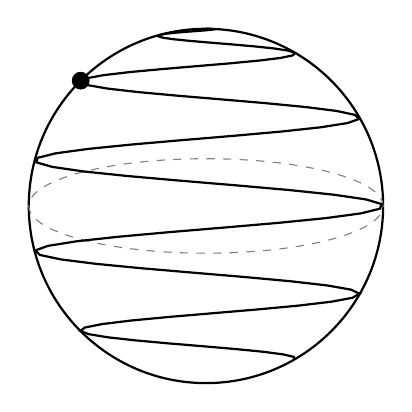
\begin{tikzpicture}[scale=1.5]
        % --- 1. Esfera (Contorno) ---
        \draw[thick] (0,0) circle (1.5);
        \draw[dashed, gray] (0,0) ellipse (1.5 and 0.4); % Ecuador

        % --- 2. Dibujo de la Espiral (Simulada) ---
        \draw[thick, samples=100, domain=0:10*pi] 
            plot ({1.5*sin(deg(\x/12))*cos(deg(\x))}, {1.5*cos(deg(\x/12))});
            
        % --- 3. Partícula ---
        \filldraw ({1.5*sin(deg(pi/4))*cos(deg(3*pi))}, {1.5*cos(deg(pi/4))}) circle (2pt);
    \end{tikzpicture}
    \caption{Trayectoria espiral sobre una superficie esférica de radio $R$.}
\end{figure}